\documentclass[11pt,aspectratio=169]{beamer}

\geometry{paperwidth=160mm,paperheight=120mm}

\usetheme[{titleformat plain}=smallcaps,
           titleformat title=smallcaps,
           titleformat subtitle=regular,
           titleformat section=smallcaps,
           titleformat frame=smallcaps,
        %    numbering=fraction,
          ]{metropolis}

\usepackage{style/main}
\usepackage[T1]{fontenc}
\usepackage[english]{babel}
\usepackage{graphicx}
\usepackage{tcolorbox}
\usepackage{xcolor}
\usepackage{amsmath,bm,amsfonts,amssymb,array,calc,amsthm,rotating,amscd,bbm}
\usepackage{url}
\usepackage{hyperref}
\usepackage{fontawesome}
\usepackage{movie15}
\usepackage{tikz}
\usepackage{multicol}
\usepackage{wrapfig}
\usetikzlibrary{quantikz}
\setbeamercolor{background canvas}{bg=white}

% in documenet


\usefonttheme[onlymath]{serif}
\usepackage[absolute,overlay]{textpos}

\setbeamerfont{caption}{size=\scriptsize}
% \usepackage[natbib=true,backend=biber,useprefix=true]{biblatex}
% \addbibresource{references.bib}
% \setbeamercolor{bibliography item}{parent=palette primary}
% \setbeamercolor*{bibliography entry title}{parent=palette primary}

% \usetheme[progressbar=frametitle]{metropolis}
% \setbeamertemplate{frame numbering}[fraction]
% \metroset{background=dark}
% \definecolor{primary}{RGB}{245, 10, 10}
% \setbeamercolor{palette primary}{bg=white, fg=black}
% \setbeamercolor{background canvas}{parent=palette primary}
% \setbeamercolor{normal text}{fg=black}
% \setbeamercolor{progress bar}{use=palette primary, fg=primary}
% natbib=true,style=authoryear,backend=bibtex,useprefix=true
% \setbeamerfont{caption}{size=\tiny}

% \usepackage[style=authoryear]{biblatex}
%%% THIS ADDS THE COMMA BETWEEN AUTHOR NAME AND YEAR
% \renewcommand*{\nameyeardelim}{\addcomma\space}
% \addbibresource{test.bib}


\title{Style-based quantum generative adversarial networks for Monte Carlo events}
\subtitle{\scriptsize C. Bravo-Prieto, J. Baglio, M. C`e, A. Francis, D. M. Grabowska and S. Carrazza - Quantum 6, 777 (2022)}
\author{Andrea Pasquale on the behalf of Stefano Carrazza}
\date{13th October 2022}
\titlegraphic{
    \vspace*{11.5cm}
    \raisebox{20pt}[10pt][10pt]{
\includegraphics[height=4cm]{../logos/unimi_logo.pdf}}\hspace*{30pt}
    \raisebox{20pt}[10pt][10pt]{
\includegraphics[height=4cm]{../logos/tii_logo.png}}\hspace*{30pt}
    \raisebox{20pt}[10pt][10pt]{
\includegraphics[height=4cm]{../logos/infn_logo.png}}\hspace*{30pt}
    % \includegraphics[height=1.3cm]{../_logos/erc_logo1.png}

    % \vfill\vspace*{230pt}
    % 
\includegraphics[height=1cm]{../_logos/unimi_logo.png}\hfill
    % 
\includegraphics[height=1cm]{../_logos/infn_logo.png}\\
    % \vspace*{5pt}
    % {
    %     \fontsize{3pt}{3.5pt}\selectfont
    %     \begin{center}
    %         This project has received funding from the European Union's Horizon
    %         2020 research and innovation programme under grant agreement No
    %         % 740006\quad \includegraphics[height=5pt]{../_logos/eu-flag.jpg}
    %     \end{center}
    % }
}
\setbeamertemplate{section in toc}[square]

\begin{document}

\maketitle

\begin{frame}{Outline}
\tableofcontents
\end{frame}
\section{Problem: event generation at LHC}

\begin{frame}{Hadronic collisions at the LHC}
    Monte Carlo event simulation is {\color{red}\textbf{very intensive}} and requires lots of {\color{blue}\textbf{computational power}}.
    \begin{figure}
        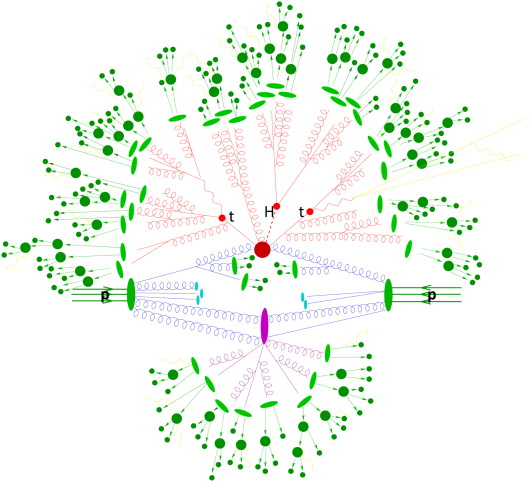
\includegraphics[width=0.6 \textwidth]{figures/sherpa-sim.jpg}
    \end{figure}
\end{frame}

\begin{frame}{Machine learning approach to event generation}
    Since 2018, many papers have approached event generation with machine learning techniques:
    \begin{figure}
        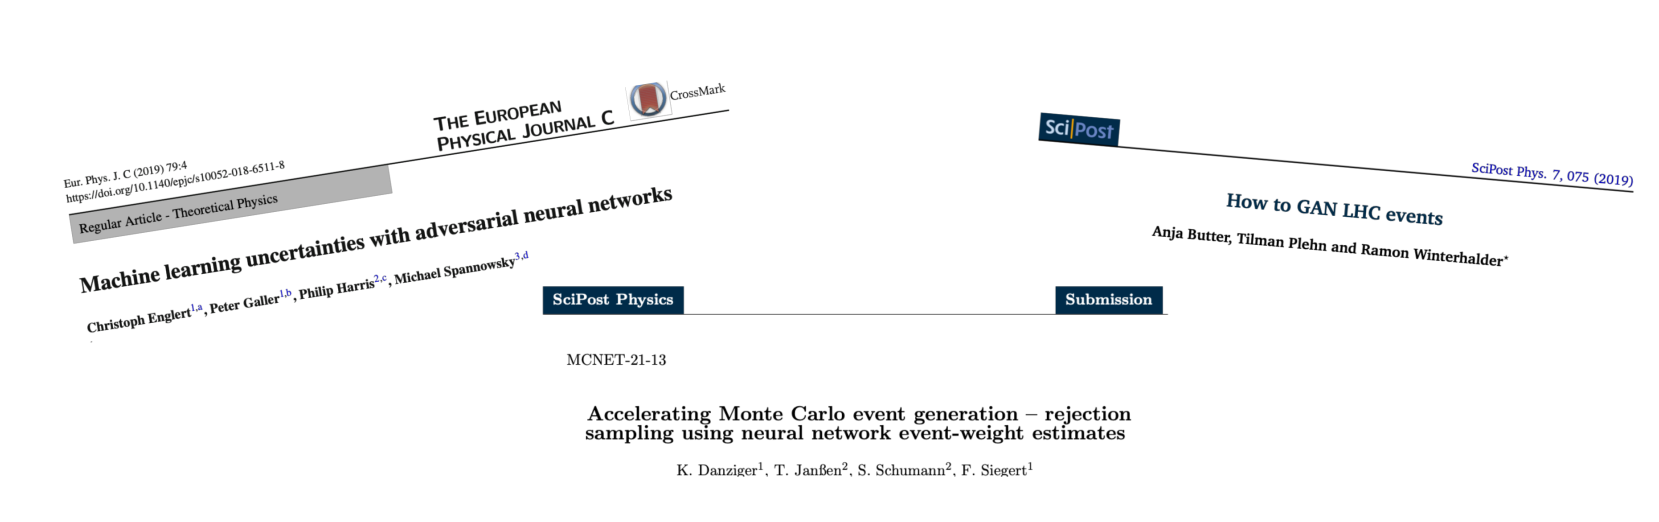
\includegraphics[width=\textwidth]{figures/ml_papers.png}
    \end{figure}
    General approach:
    \begin{enumerate}
        \item Train unsupervised models on \textbf{small} dataset to learn underlying pdf
        \item Generate \textbf{more data} using those models $\Rightarrow$ data augmentation
    \end{enumerate}
    
\end{frame}
\section{Methodology}

\begin{frame}{Unsupervised Learning: Generative Adversarial Networks}
    \textbf{Two networks competing}: generator produces \textbf{fake} data, while the discriminator
distinguishes between \textbf{real} input data and fake data (produced by the generator).
\begin{figure}
    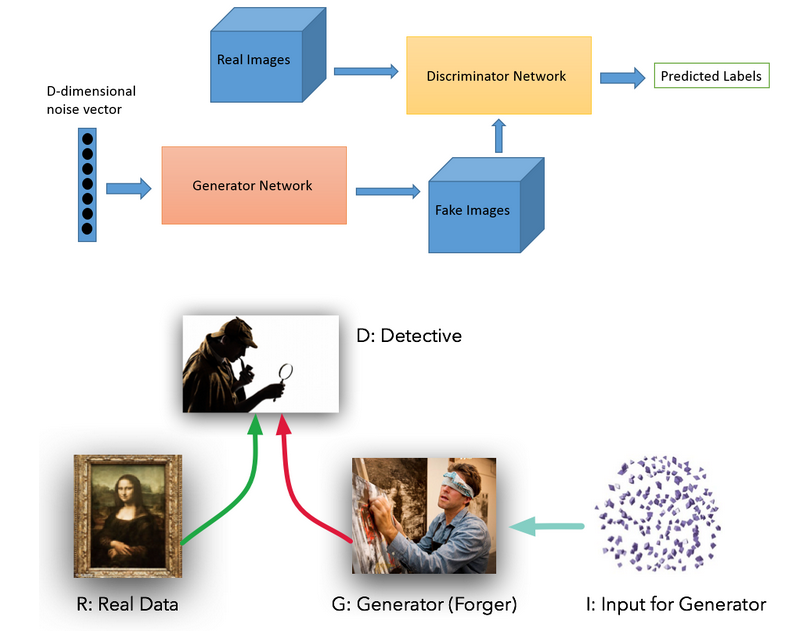
\includegraphics[width=0.8 \textwidth]{figures/gan_image.jpg}
\end{figure}
    
\end{frame}

% \begin{frame}{Unsupervised Learning: Generative Adversarial Networks}
%     Adversarial game where the generator learns to map input noise to the underlying distribution:
%     \begin{figure}
%         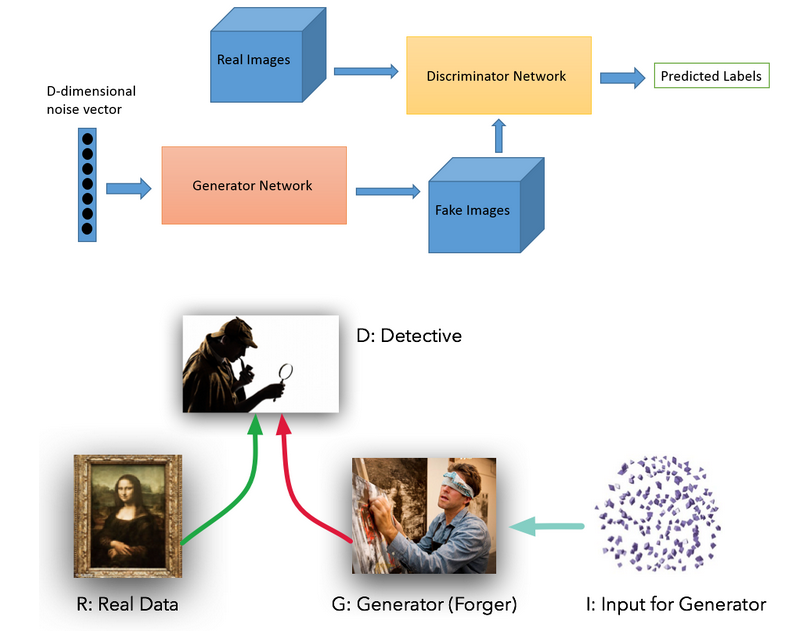
\includegraphics[width=0.8 \textwidth]{figures/gan_image.jpg}
%     \end{figure}
% \end{frame}


\begin{frame}{Training procedure}
    \textbf{Training}: adapt alternatively the generator $G(\phi_g , z)$ and the discriminator $D(\phi_d , x)$
    \textbf{Metrics}: binary cross-entropy for the loss functions:
    \begin{itemize}
        \item Generator loss function:
        $$ \mathcal{L}_G(\phi_g,\phi_d) = -\mathbb{E}_{z \sim p_{\mathrm{prior}}(z)}[\log D(\phi_d,G(\phi_g,z))]  $$
        \item Discriminator loss function:
        $$ \mathcal{L}_D(\phi_g,\phi_d) = \mathbb{E}_{x \sim p_{\mathrm{real}}(x)}[\log D(\phi_d,x)] +\, \mathbb{E}_{z \sim p_{\mathrm{prior}}(z)}[\log (1-D(\phi_d,G(\phi_g,z)))]\,.$$
    \end{itemize}
 
    \textbf{Game theory}: min-max two-player game to reach Nash equilibrium
    $$ \underset{\phi_g}{\min}\,\,\mathcal{L}_G(\phi_g,\phi_d)  \quad  \underset{\phi_d}{\max}\,\,\mathcal{L}_D(\phi_g,\phi_d) $$
   
    % \begin{columns}
    %     \begin{column}{0.5 \textwidth}
    %         Training procedure
    %     \end{column}

    %     \begin{column}{0.5 \textwidth}
    %         Training procedure
    %     \end{column}
    % \end{columns}
   
\end{frame}

\begin{frame}{Machine learning with quantum computing?}
    Can we develop an efficient GAN-like model for event generation using quantum hardware?
    
    Why Quantum ML?
    \begin{itemize}
        \item Proof-of-concept, study new architectures. 
        \begin{itemize}
            \item fast inference (native representation / sampling)?
            \item fast training / compact models with few parameters?
        \end{itemize}
        \item Obtain a hardware representation (analogy with GPU and FPGA).
        \item Lower power consumption.
    \end{itemize}

\end{frame}

\begin{frame}{Hybrid approach }
    \begin{figure}
        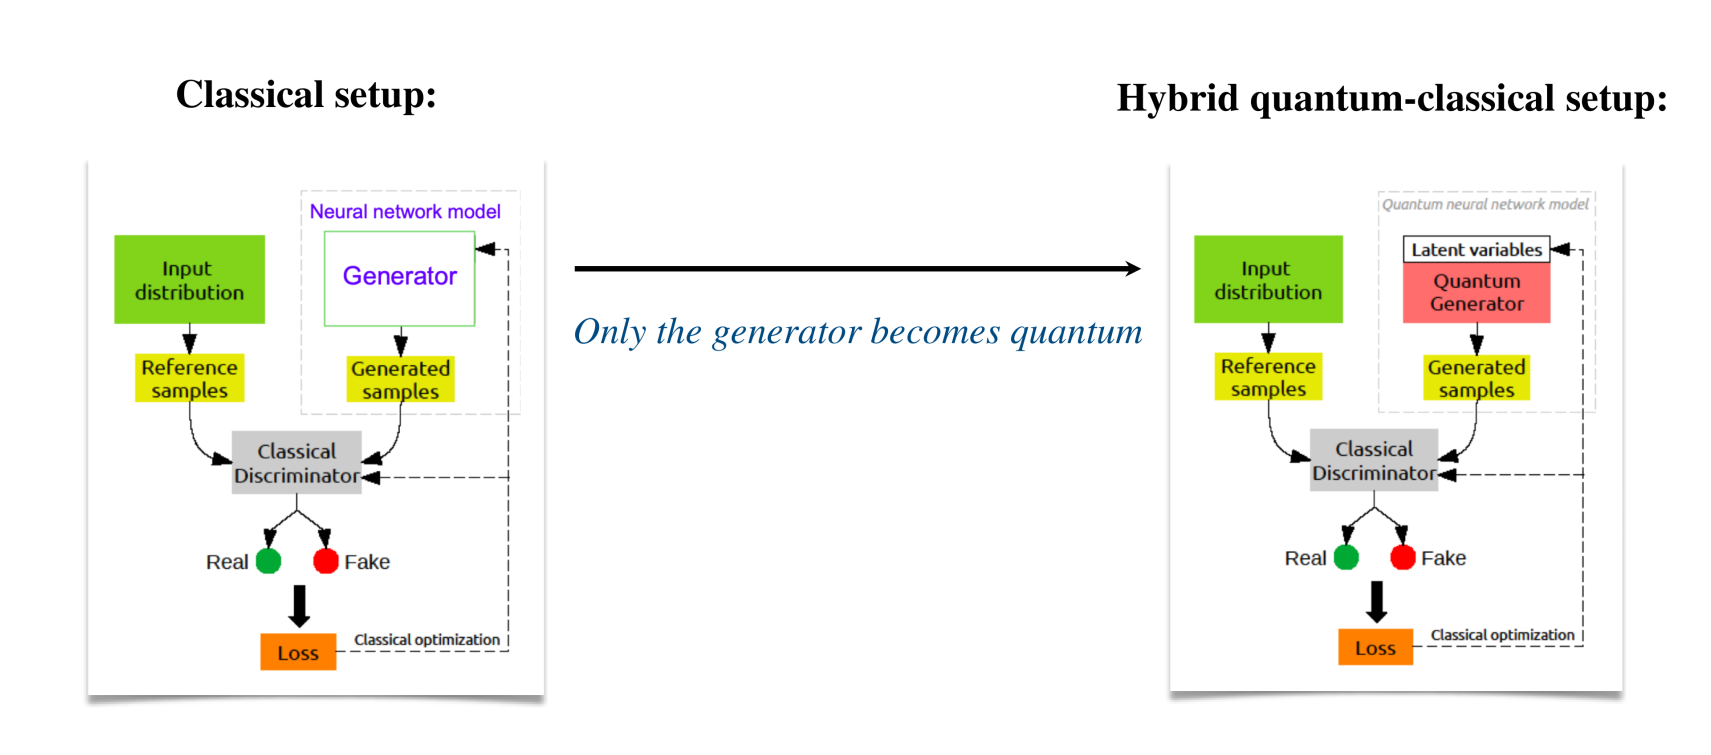
\includegraphics[width=1\textwidth]{figures/qGAN.png}
    \end{figure}
\end{frame}

\begin{frame}{Style-based quantum generator}
    \textbf{Quantum generator}: a series of quantum layers with rotation and entanglement gates
    \vspace{0.5cm}

    % \begin{columns}
    %     \begin{column}{0.6 \textwidth}
        \centering
            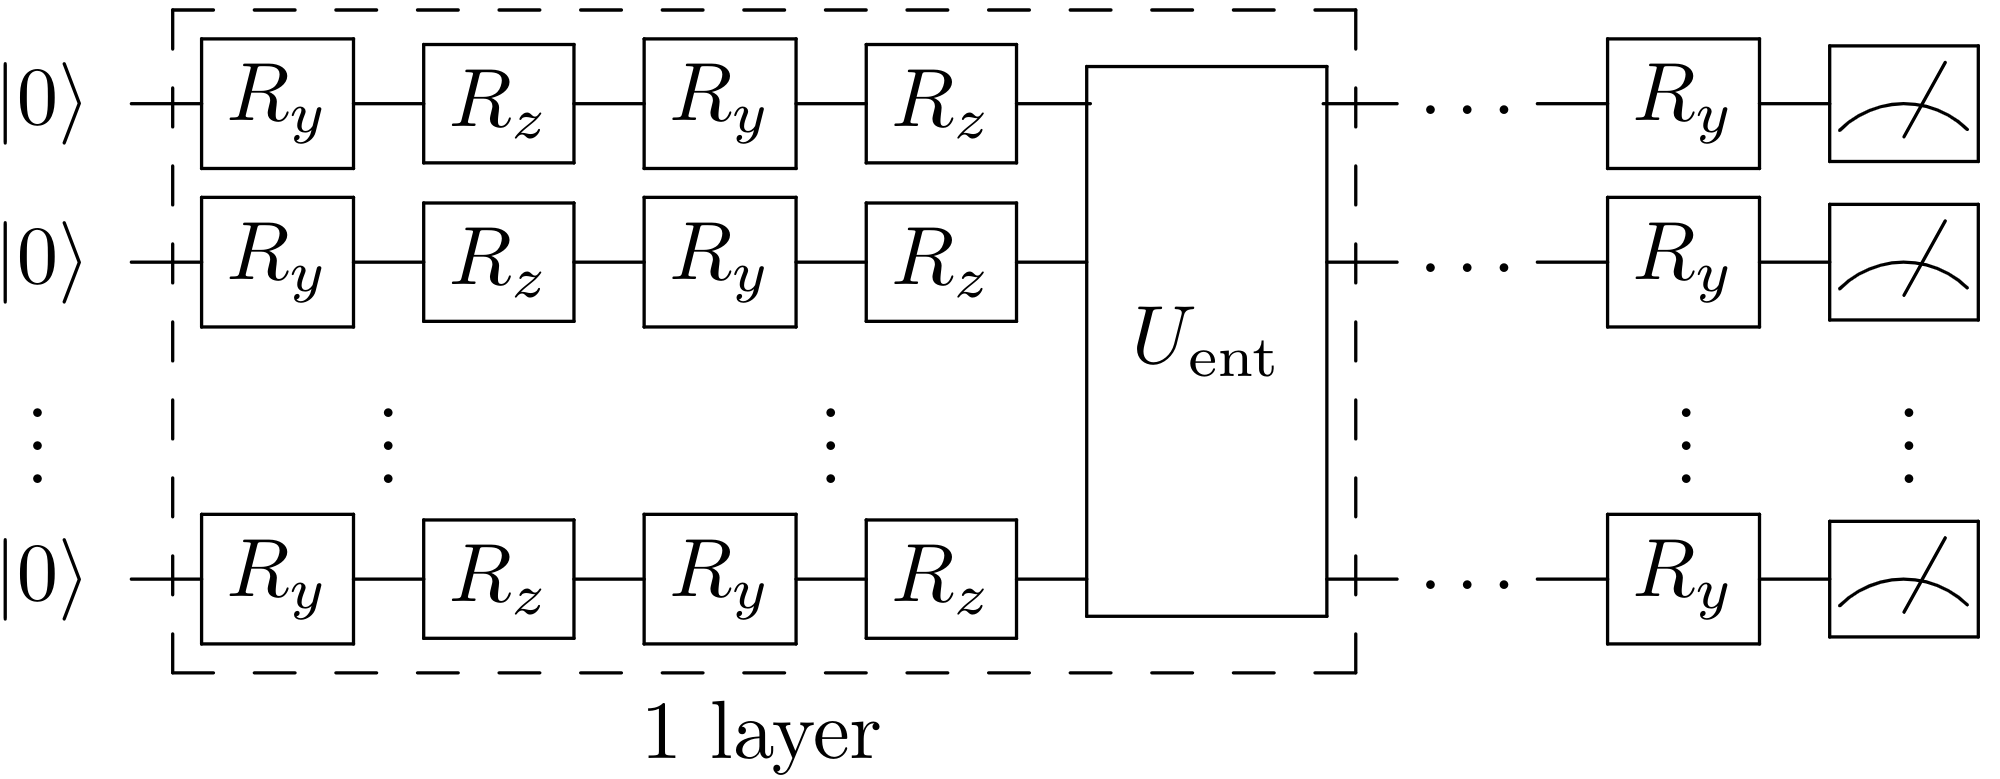
\includegraphics[width=0.7\textwidth]{figures/ansatz.png}
        % \end{column}
        % \begin{column}{0.4 \textwidth}
        %     1 component = 1 qubit
            
        %     $$ \textbf{x} = ( - \expval{\sigma_z^1}, \ldots , - \expval{\sigma_z^n})$$
            
        % \end{column}
    % \end{columns}
    \begin{tcolorbox}[title=Style-based approach]
        The noise is inserted in every gate and not only in the initial quantum state
        \[ R_{y,z}^{l,m}(\vec{\phi}_g, \vec{z}) = R_{y,z}(\phi_g^{(l)} z^{(m)} + \phi_g^{(l-1)}) \]
        
    \end{tcolorbox}
\end{frame}
\section{Results}

\begin{frame}{Validation: 1D Gamma distribution}
    \textbf{Assessing the validity of the approach}: train and test on known toy model distribution
    
    With 1 qubit, one layer, using 100 bins: 1D Gamma function
    $$ p_\gamma (x, \alpha, \beta) = x^{\alpha-1} \frac{e^{-x/\beta}}{\beta^\alpha \Gamma (\alpha)}$$
    \begin{multicols*}{2}
        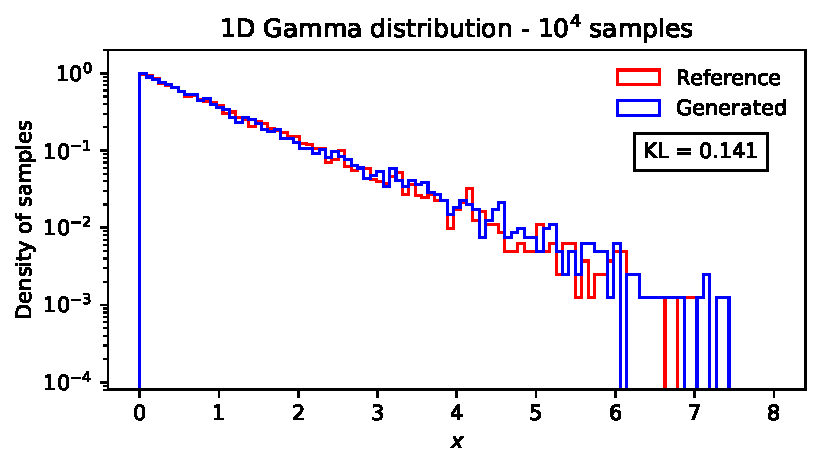
\includegraphics[width=0.5 \textwidth]{figures/plots/1Dgamma/1Dgamma_distribution_10k.pdf}
        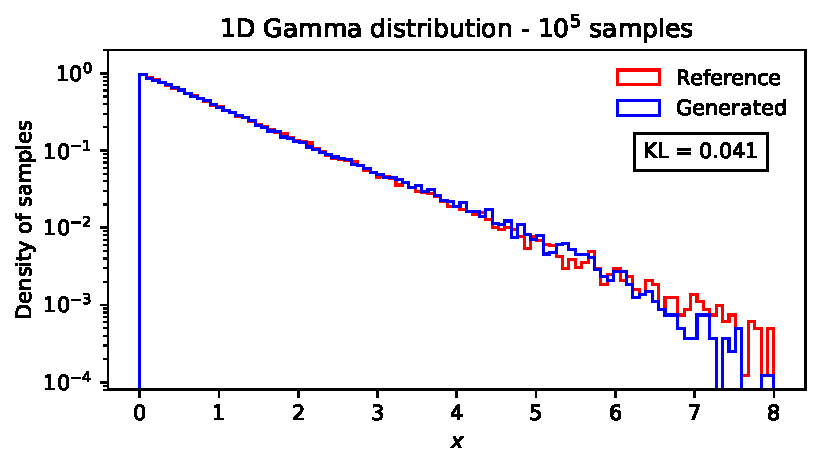
\includegraphics[width=0.5 \textwidth]{figures/plots/1Dgamma/1Dgamma_distribution_100k.pdf}
    \end{multicols*}
    \begin{itemize}
        \item Train on $10^4$ samples until convergence is reached.
        \item Use generator to generate $10^4$ and $10^5$ samples to demonstrate data augmentation
    \end{itemize}
\end{frame}

\begin{frame}{Validation: 3D correlated Gaussian distribution}
    Test whether the style-qGAN captures correlations: train on 3D Gaussian distribution, with
    \begin{equation*}
        p(\vec{x}) \propto \exp \Big[ - \frac{1}{2} (\vec{x} - \vec{\mu})^T
        \Sigma^{-1} (\vec{x} - \vec{\mu}) \Big] \,, \quad
        \mu =
\begin{pmatrix}
  0 \\
  0 \\
  0 \\
  \end{pmatrix}\,, \quad
        \Sigma =
\begin{pmatrix}
  0.5 & 0.1 & 0.25\\
  0.1 & 0.5 & 0.1\\
  0.25 & 0.1 & 0.5\\
  \end{pmatrix}.
    \end{equation*}
    Using 3 qubits, one layer, 100 bins:
    \begin{multicols*}{3}
        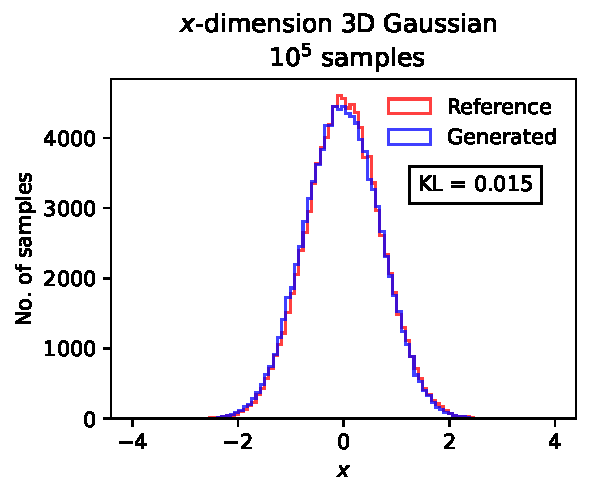
\includegraphics[width=0.33 \textwidth]{figures/plots/3Dgaussian_posdef/1-distribution_3dgaussian_100k.pdf}
        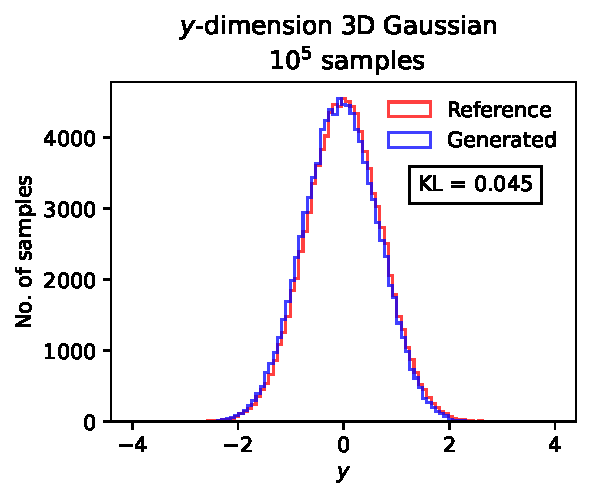
\includegraphics[width=0.33 \textwidth]{figures/plots/3Dgaussian_posdef/2-distribution_3dgaussian_100k.pdf}
        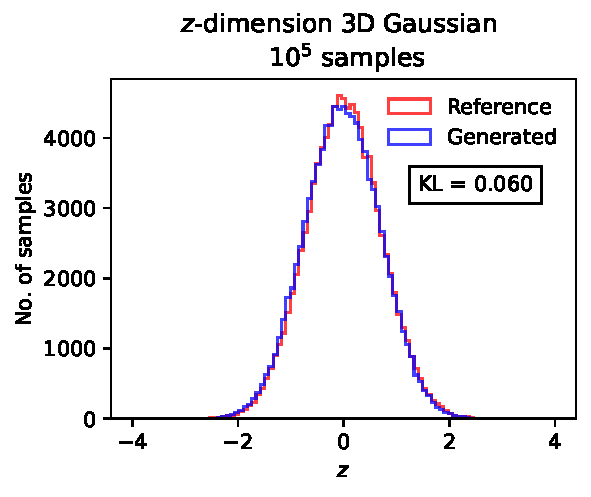
\includegraphics[width=0.33\textwidth]{figures/plots/3Dgaussian_posdef/3-distribution_3dgaussian_100k.pdf}
    \end{multicols*}
\end{frame}

\begin{frame}{Validation: 3D correlated Gaussian distribution}
    Test whether the style-qGAN captures correlations: train on 3D Gaussian distribution, with
    \begin{equation*}
        p(\vec{x}) \propto \exp \Big[ - \frac{1}{2} (\vec{x} - \vec{\mu})^T
        \Sigma^{-1} (\vec{x} - \vec{\mu}) \Big] \,, \quad
        \mu =
\begin{pmatrix}
  0 \\
  0 \\
  0 \\
  \end{pmatrix}\,, \quad
        \Sigma =
\begin{pmatrix}
  0.5 & 0.1 & 0.25\\
  0.1 & 0.5 & 0.1\\
  0.25 & 0.1 & 0.5\\
  \end{pmatrix}.
    \end{equation*}
    Using 3 qubits, one layer, 100 bins:
    \begin{multicols*}{3}
        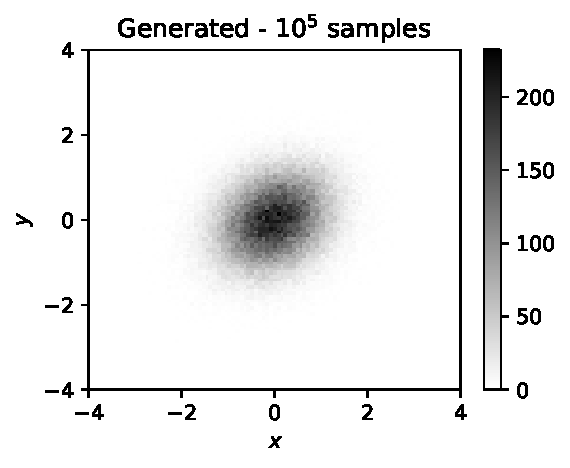
\includegraphics[width=0.33 \textwidth]{figures/plots/3Dgaussian_posdef/1-2_FAKE_100k.pdf}
        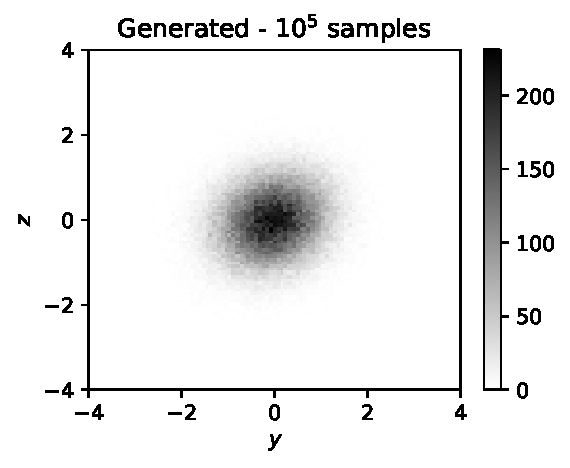
\includegraphics[width=0.33 \textwidth]{figures/plots/3Dgaussian_posdef/2-3_FAKE_100k.pdf}
        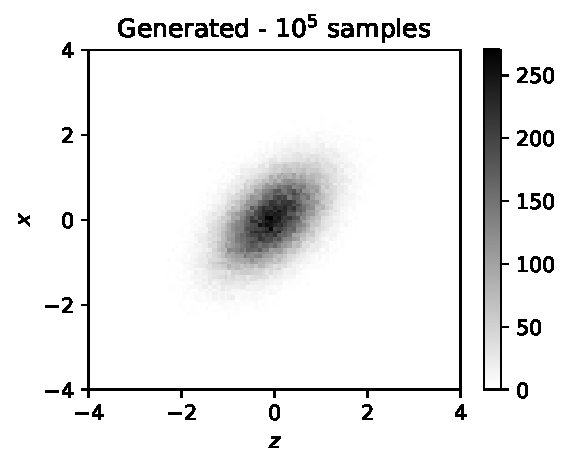
\includegraphics[width=0.33\textwidth]{figures/plots/3Dgaussian_posdef/3-1_FAKE_100k.pdf}
    \end{multicols*}
    \centering
    Correlations are well captured!
\end{frame}

\begin{frame}{Validation: 3D correlated Gaussian distribution}
    Test whether the style-qGAN captures correlations: train on 3D Gaussian distribution, with
    \begin{equation*}
        p(\vec{x}) \propto \exp \Big[ - \frac{1}{2} (\vec{x} - \vec{\mu})^T
        \Sigma^{-1} (\vec{x} - \vec{\mu}) \Big] \,, \quad
        \mu =
\begin{pmatrix}
  0 \\
  0 \\
  0 \\
  \end{pmatrix}\,, \quad
        \Sigma =
\begin{pmatrix}
  0.5 & 0.1 & 0.25\\
  0.1 & 0.5 & 0.1\\
  0.25 & 0.1 & 0.5\\
  \end{pmatrix}.
    \end{equation*}
    Using 3 qubits, one layer, 100 bins:
    \begin{multicols*}{3}
        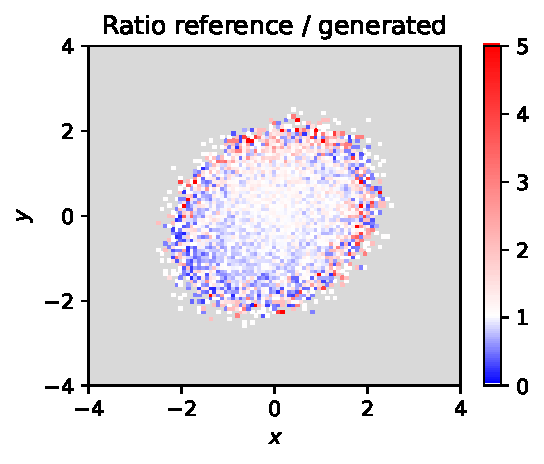
\includegraphics[width=0.33 \textwidth]{figures/plots/3Dgaussian_posdef/1-2_RATIO_100k.pdf}
        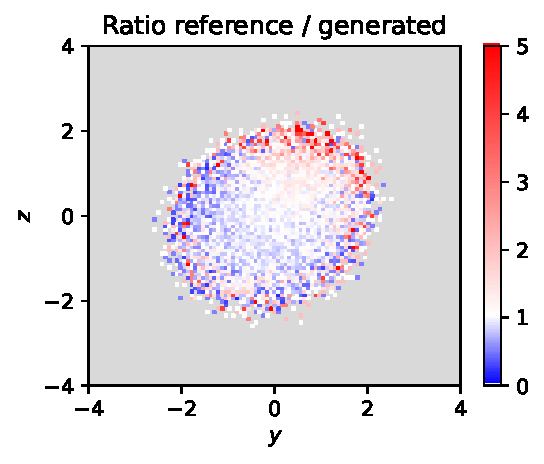
\includegraphics[width=0.33 \textwidth]{figures/plots/3Dgaussian_posdef/2-3_RATIO_100k.pdf}
        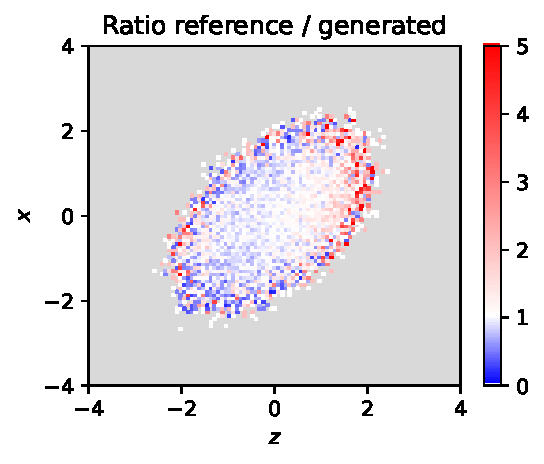
\includegraphics[width=0.33\textwidth]{figures/plots/3Dgaussian_posdef/3-1_RATIO_100k.pdf}
    \end{multicols*}
    \centering
    Correlations are well captured!
\end{frame}

\begin{frame}{Simulation with LHC data}
    Testing the style-qGAN with real data: proton-proton collision $pp \rightarrow t\bar{t}$

    \vspace{1cm}
    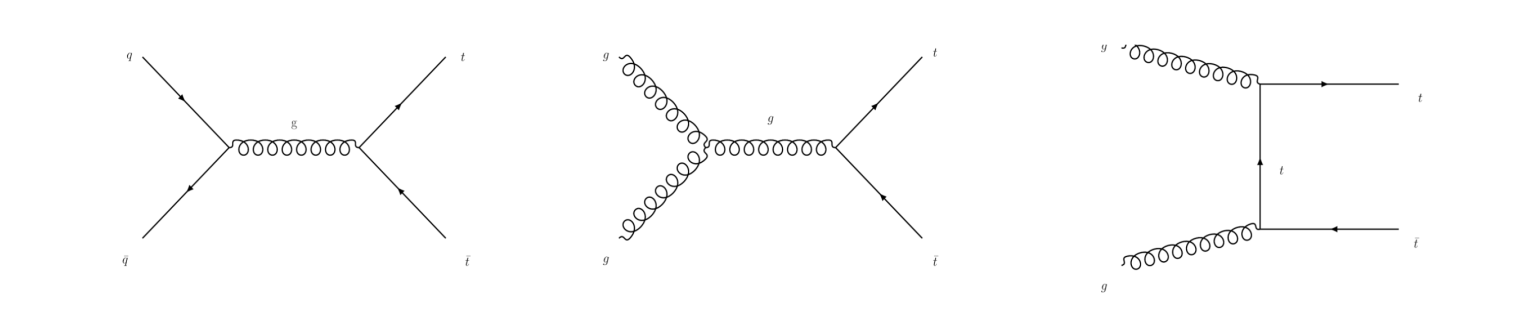
\includegraphics[width=\textwidth]{figures/ppttbar.png}

    Training and reference samples generated with MadGraph5 aMC@NLO

    Training set of $10^4$ samples, \textbf{Mandelstam variables} $(s, t)$ and rapidity $y$.
\end{frame}
% \section{Open problems}

\begin{frame}{Simulation with LHC data}
    After training, we assess the performance with simulations: 3 qubits, 2 layers, 100 bins

    \begin{multicols*}{3}
        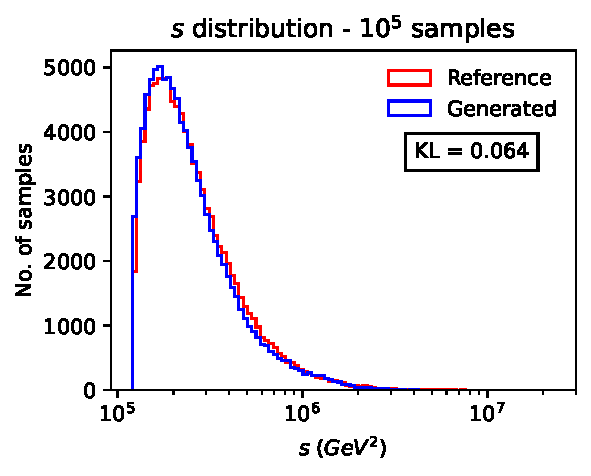
\includegraphics[width=0.33 \textwidth]{figures/plots/LHCttbar/s-distribution_LHCdata_100k.pdf}
        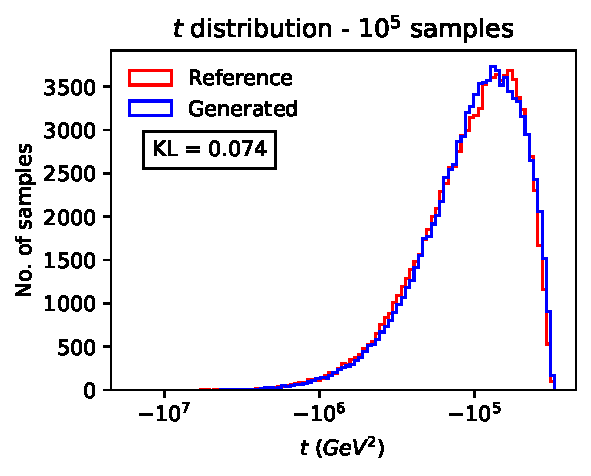
\includegraphics[width=0.33 \textwidth]{figures/plots/LHCttbar/t-distribution_LHCdata_100k.pdf}
        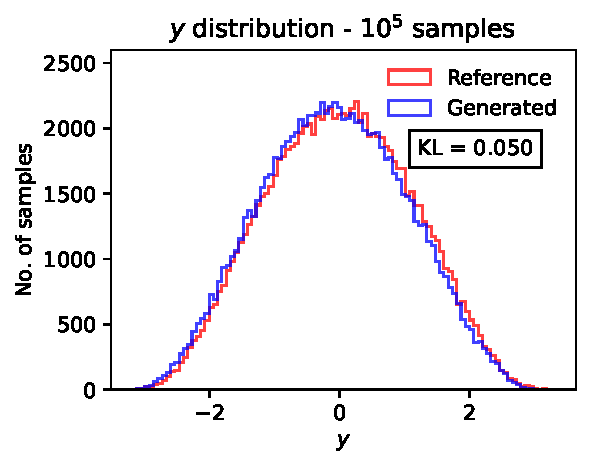
\includegraphics[width=0.33\textwidth]{figures/plots/LHCttbar/y-distribution_LHCdata_100k.pdf}
    \end{multicols*}
    \begin{center}
        {\color{red}
        \textbf{
        Remarkable low KL divergences with data augmentation!}
        }
    \end{center}
\end{frame}


% \section{Open problems}

\begin{frame}{Simulation with LHC data}
    After training, we assess the performance with simulations: 3 qubits, 2 layers, 100 bins

    \begin{multicols*}{3}
        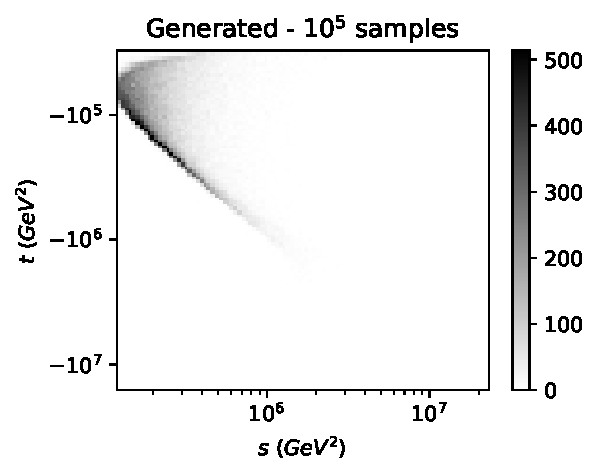
\includegraphics[width=0.33 \textwidth]{figures/plots/LHCttbar/s-t_FAKE_100k.pdf}
        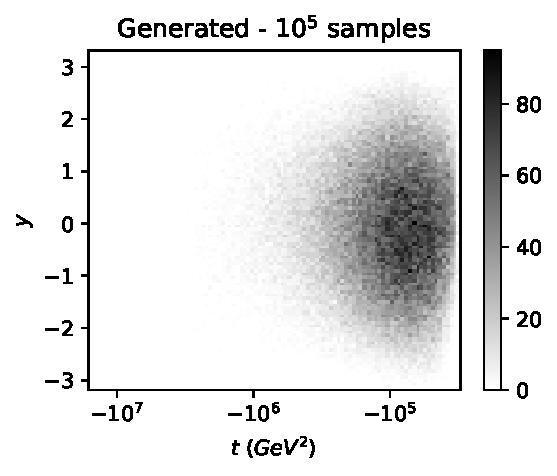
\includegraphics[width=0.33 \textwidth]{figures/plots/LHCttbar/t-y_FAKE_100k.pdf}
        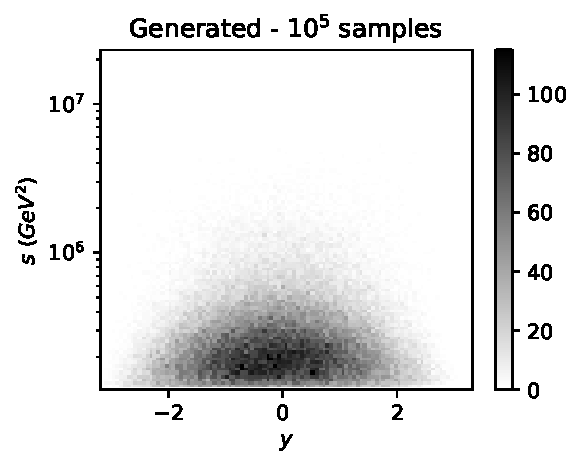
\includegraphics[width=0.33\textwidth]{figures/plots/LHCttbar/y-s_FAKE_100k.pdf}
    \end{multicols*}
    \begin{center}
        { \color{red}
        \textbf{
        Correlations are well captured!}
        }
    \end{center}
\end{frame}

\begin{frame}{Simulation with LHC data}
    After training, we assess the performance with simulations: 3 qubits, 2 layers, 100 bins

    \begin{multicols*}{3}
        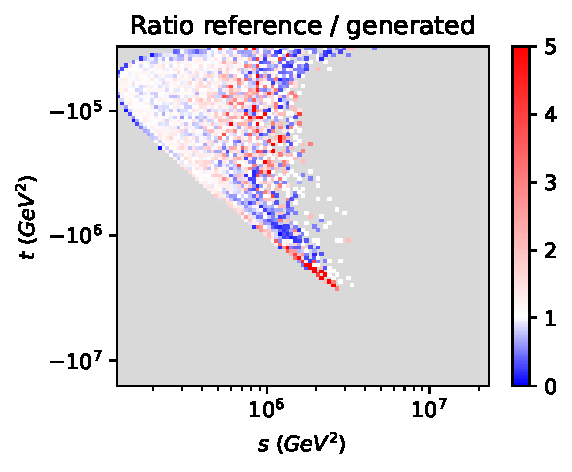
\includegraphics[width=0.33 \textwidth]{figures/plots/LHCttbar/s-t_RATIO_100k.pdf}
        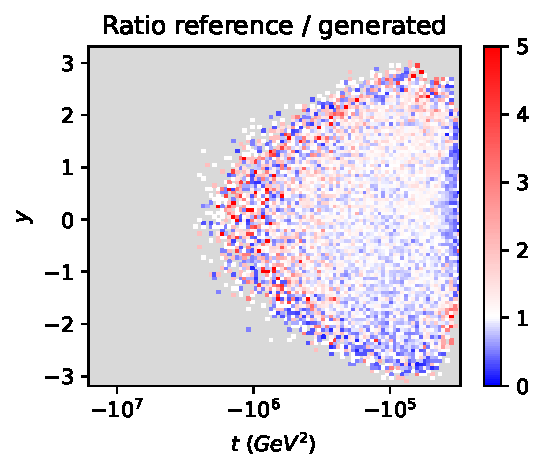
\includegraphics[width=0.33 \textwidth]{figures/plots/LHCttbar/t-y_RATIO_100k.pdf}
        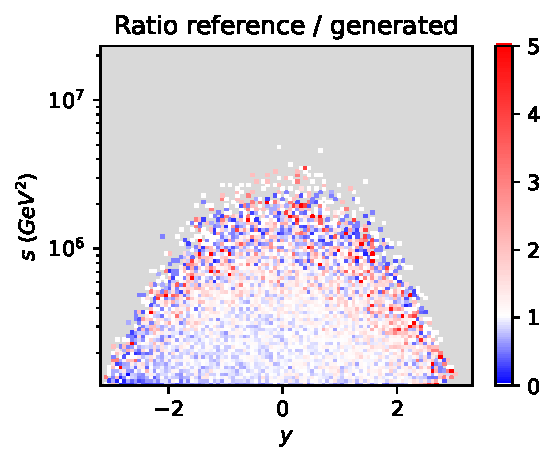
\includegraphics[width=0.33\textwidth]{figures/plots/LHCttbar/y-s_RATIO_100k.pdf}
    \end{multicols*}
    \begin{center}
        { \color{red}
        \textbf{
            Are these results maintained on real hardware?}
        }
    \end{center}
    
\end{frame}

\begin{frame}{Qibo}
    Qibo is an \textbf{open-source} full stack API for quantum simulation and quantum hardware control and calibration.
    \begin{figure}
        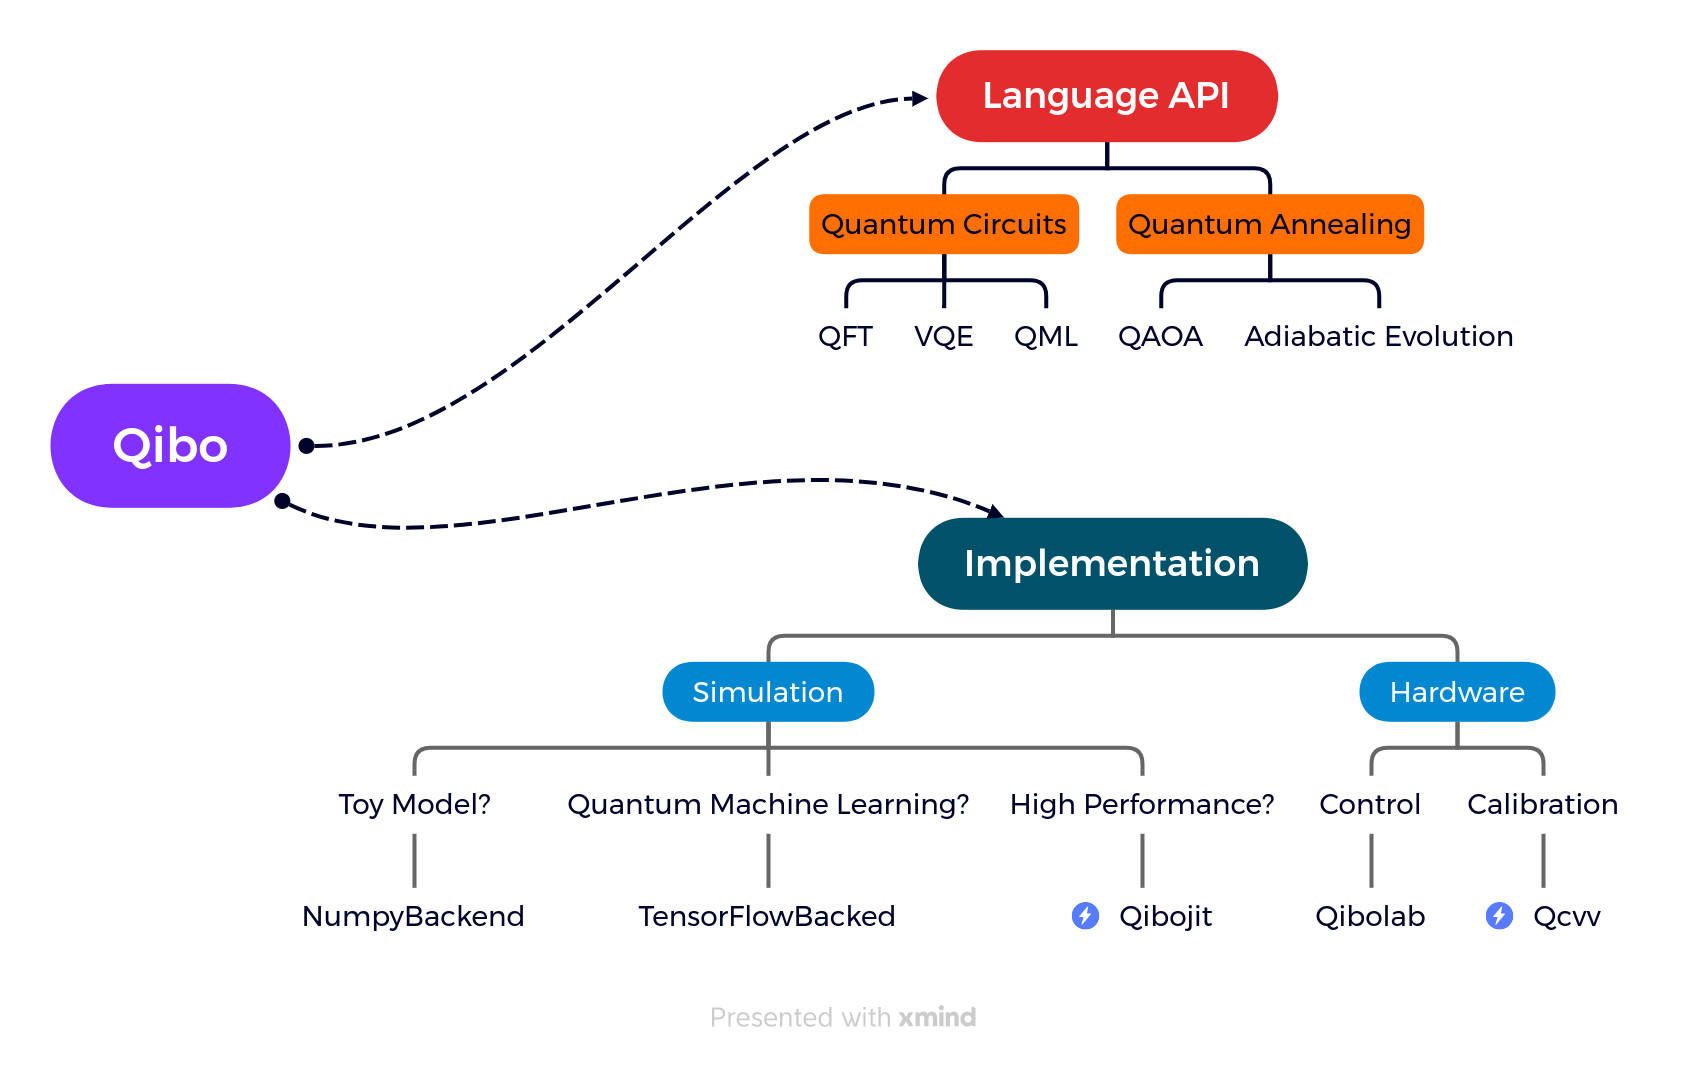
\includegraphics[width= \textwidth]{figures/Qibo.png}
    \end{figure}
\end{frame}

\begin{frame}{Qibo}

        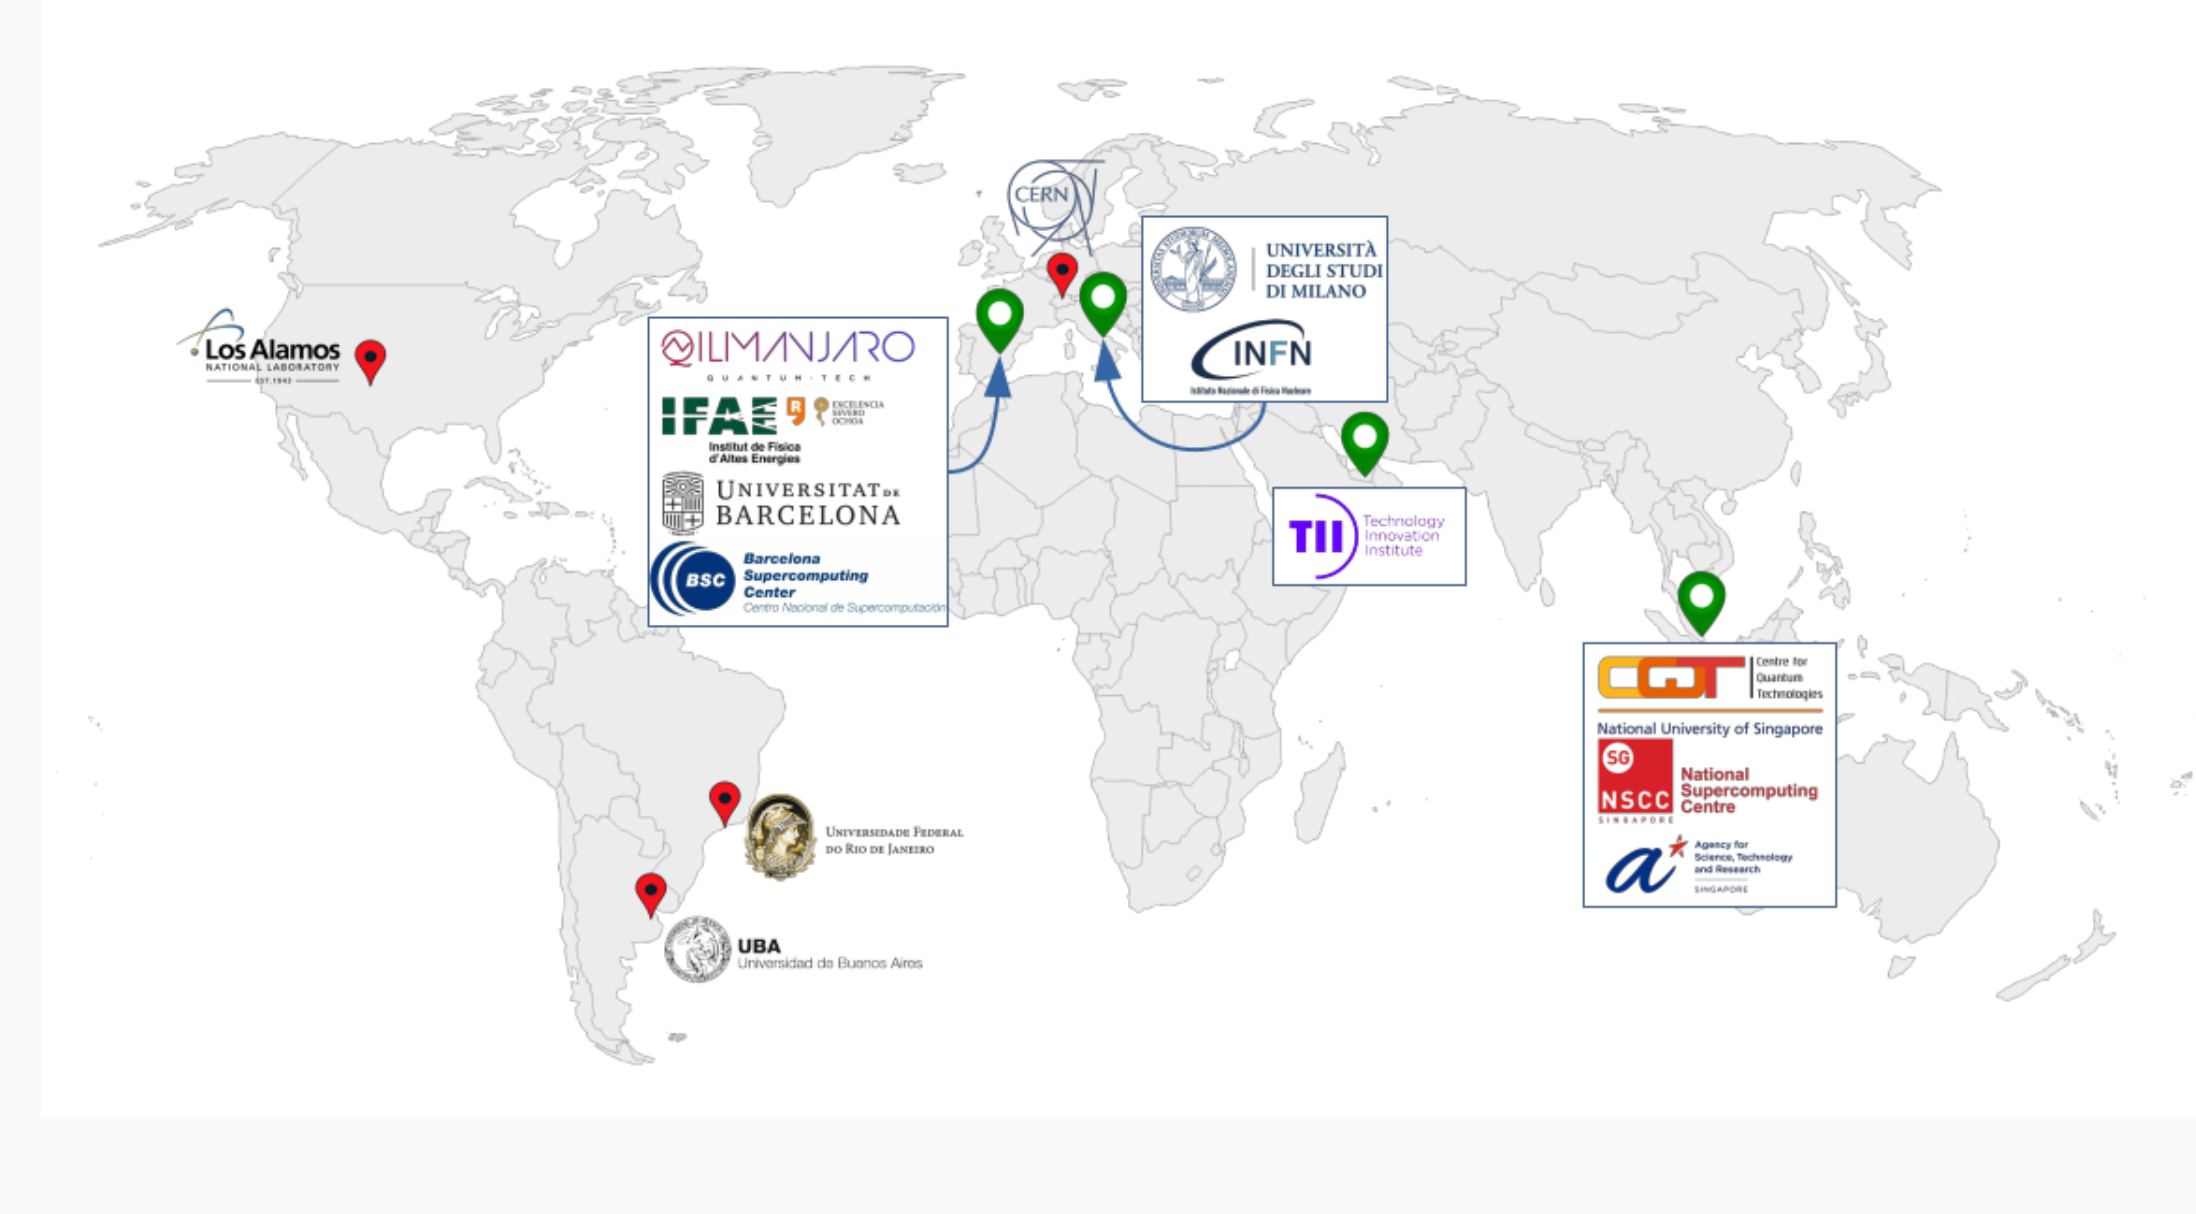
\includegraphics[width= 0.8\textwidth]{figures/map.png}

        
    
\end{frame}

\section{Result on Quantum Hardware}

\begin{frame}{Testing different architectures}
    \begin{figure}
        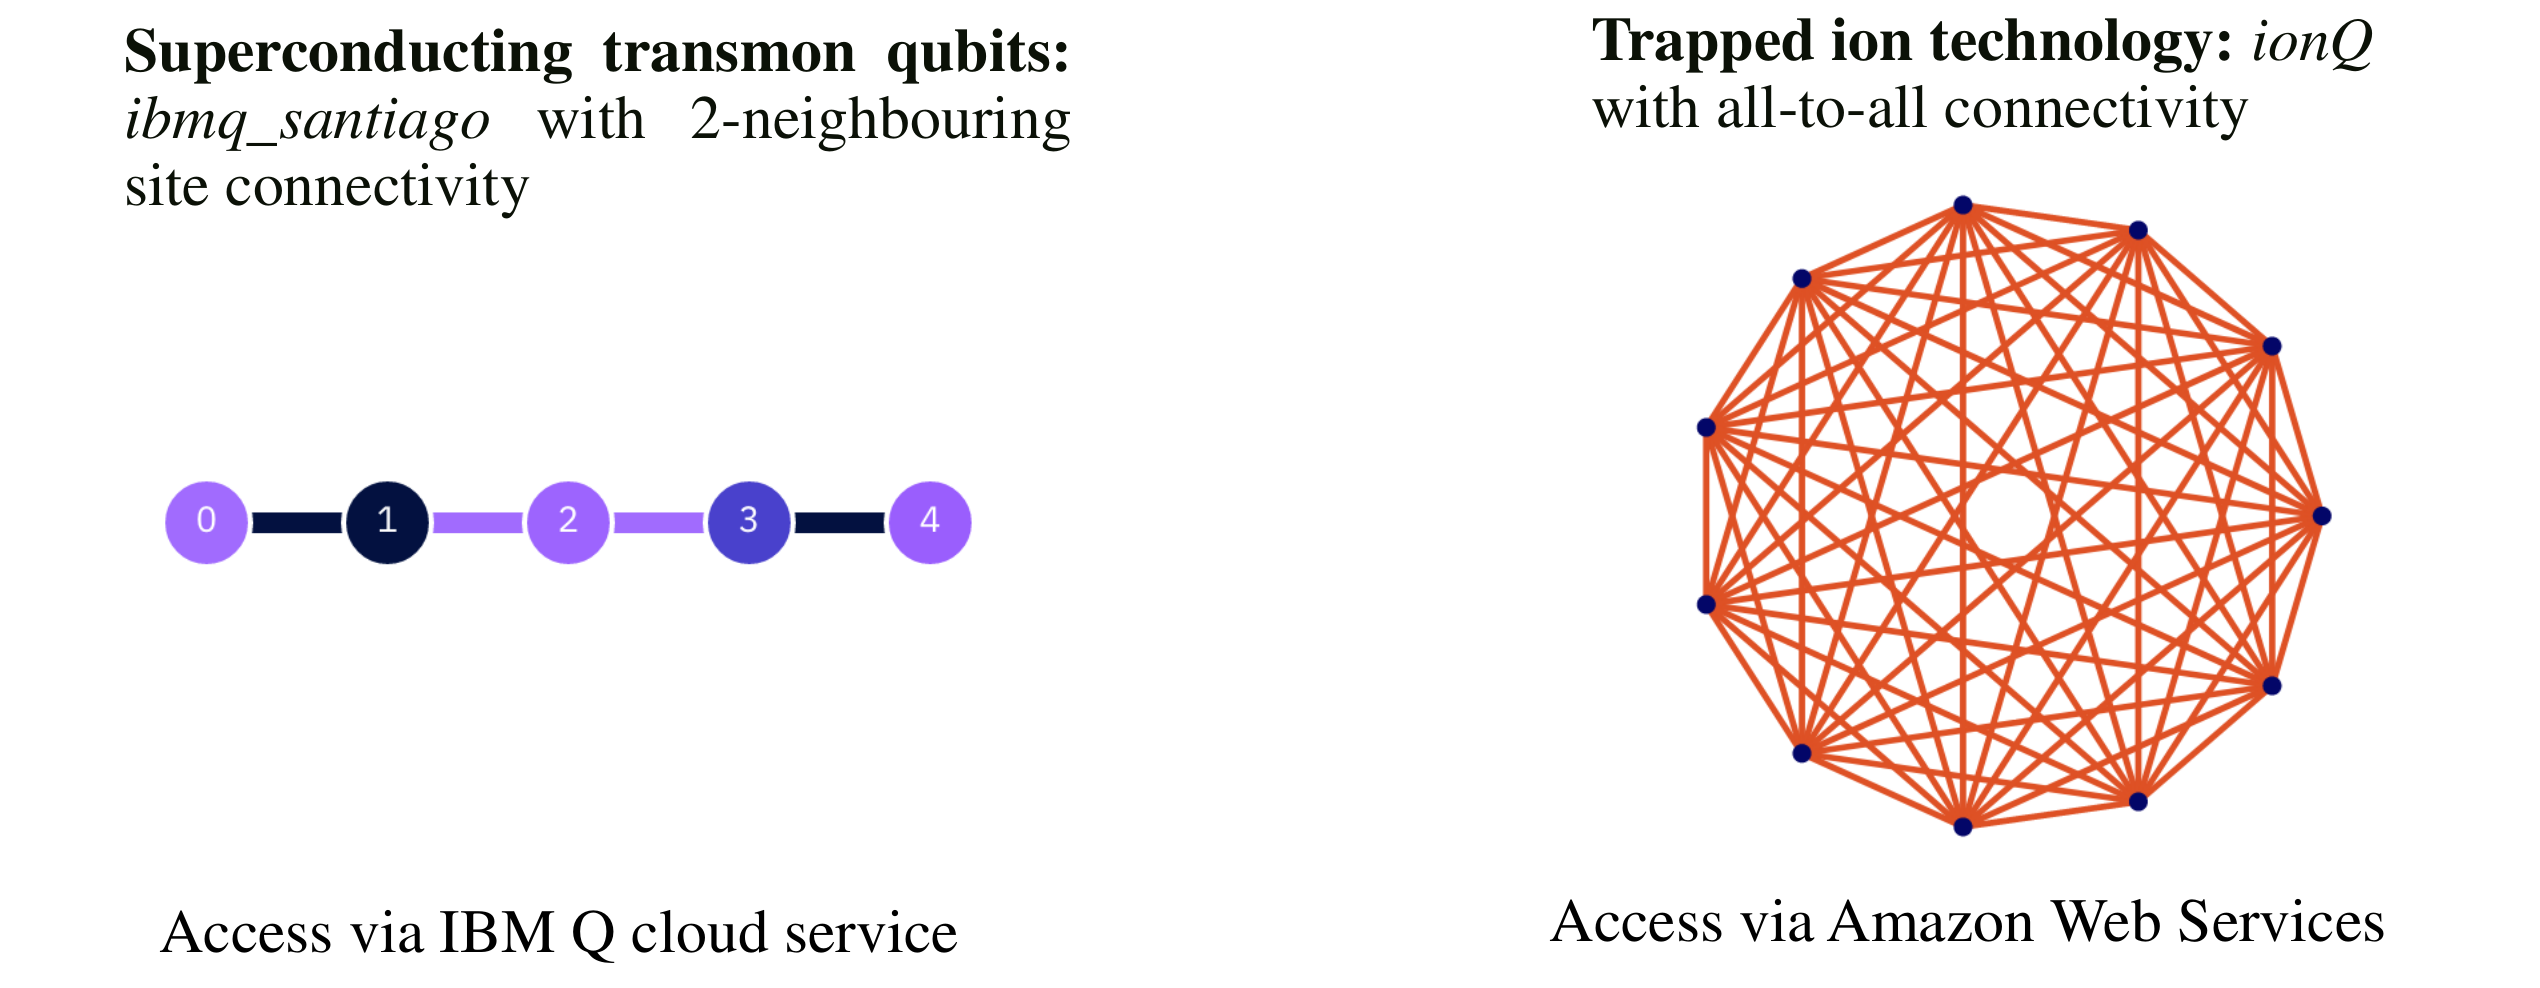
\includegraphics[width=\textwidth]{figures/ibm.png}
    \end{figure}
       
        


\end{frame}
\begin{frame}{Results on IBM Q hardware}
    \begin{multicols*}{2}
        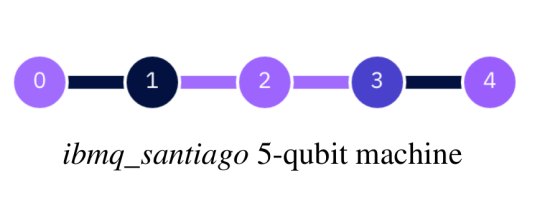
\includegraphics[width=0.37 \textwidth]{figures/ibm5q.png}
        \begin{tcolorbox}
            Still relatively low KL divergence!
        \end{tcolorbox}
    \end{multicols*}
    \begin{multicols*}{3}
        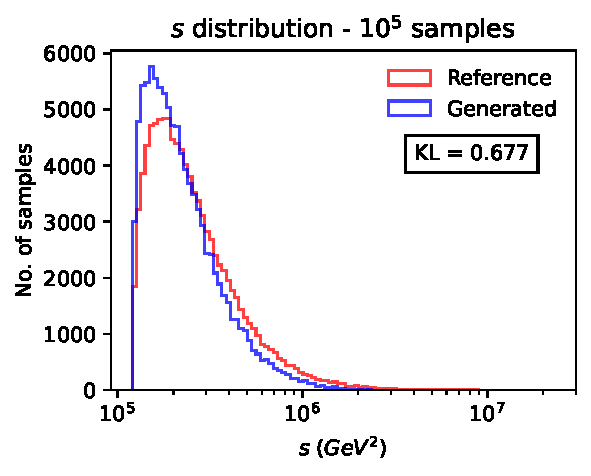
\includegraphics[width=0.33 \textwidth]{figures/plots/hardware/ibm_santiago/s-distribution_IBM_LHCdata_100k.pdf}
        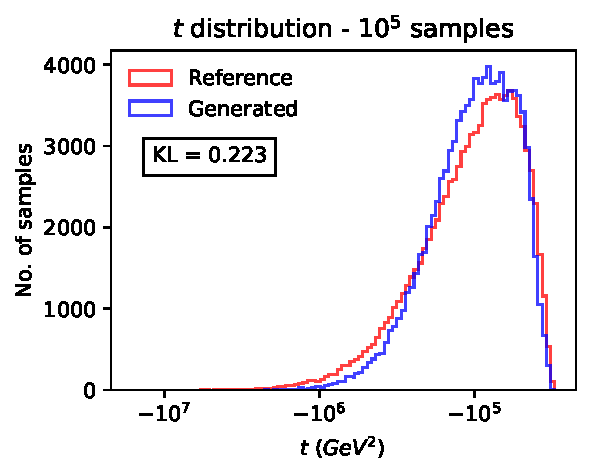
\includegraphics[width=0.33 \textwidth]{figures/plots/hardware/ibm_santiago/t-distribution_IBM_LHCdata_100k.pdf}
        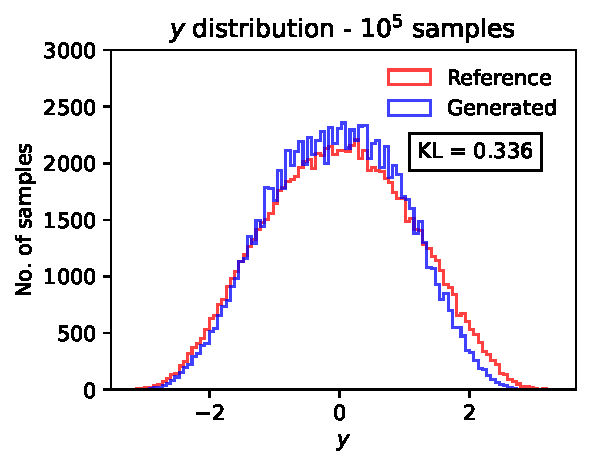
\includegraphics[width=0.33\textwidth]{figures/plots/hardware/ibm_santiago/y-distribution_IBM_LHCdata_100k.pdf}
    \end{multicols*}
\end{frame}

\begin{frame}{Results on IBM Q hardware}
    \begin{multicols*}{2}
        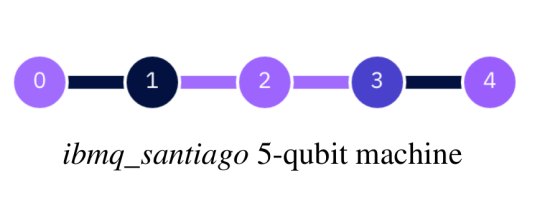
\includegraphics[width=0.37 \textwidth]{figures/ibm5q.png}
        \begin{tcolorbox}
           Correlations captured on a quantum hardware!
        \end{tcolorbox}
    \end{multicols*}
    \begin{multicols*}{3}
        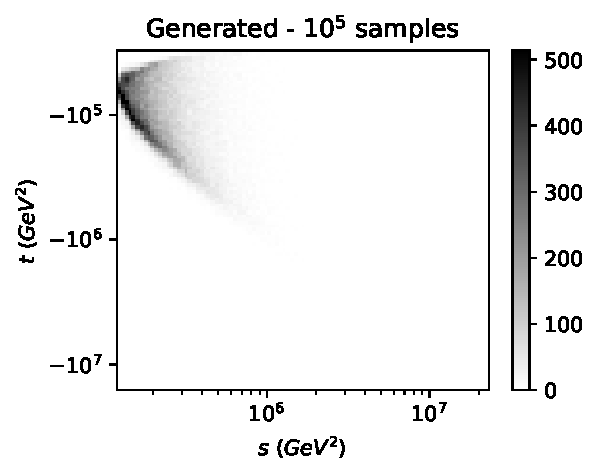
\includegraphics[width=0.33 \textwidth]{figures/plots/hardware/ibm_santiago/s-t_FAKE_IBM_100k.pdf}
        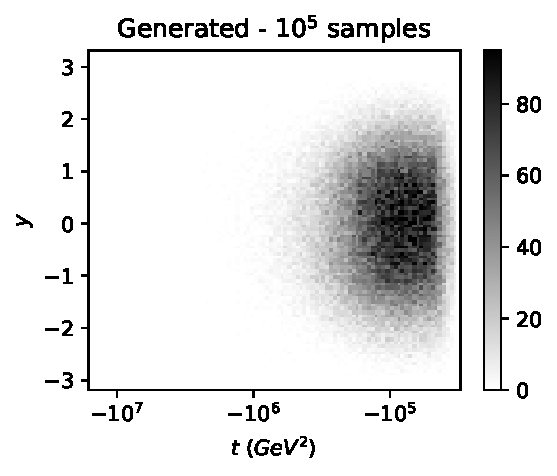
\includegraphics[width=0.33 \textwidth]{figures/plots/hardware/ibm_santiago/t-y_FAKE_IBM_100k.pdf}
        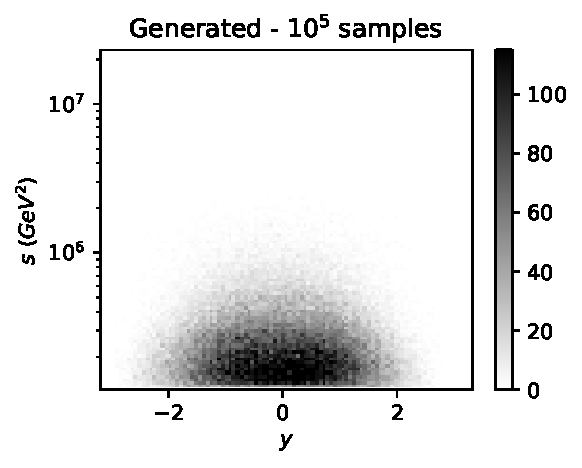
\includegraphics[width=0.33\textwidth]{figures/plots/hardware/ibm_santiago/y-s_FAKE_IBM_100k.pdf}
    \end{multicols*}
\end{frame}

\begin{frame}{Results on IBM Q hardware}
    \begin{multicols*}{2}
        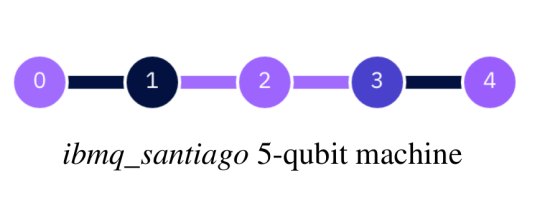
\includegraphics[width=0.37 \textwidth]{figures/ibm5q.png}
        \begin{tcolorbox}
            Still a good ratio!
        \end{tcolorbox}
    \end{multicols*}
    \begin{multicols*}{3}
        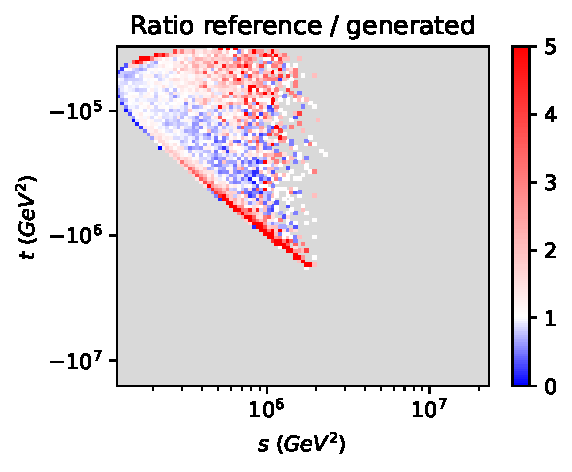
\includegraphics[width=0.33 \textwidth]{figures/plots/hardware/ibm_santiago/s-t_RATIO_IBM_100k.pdf}
        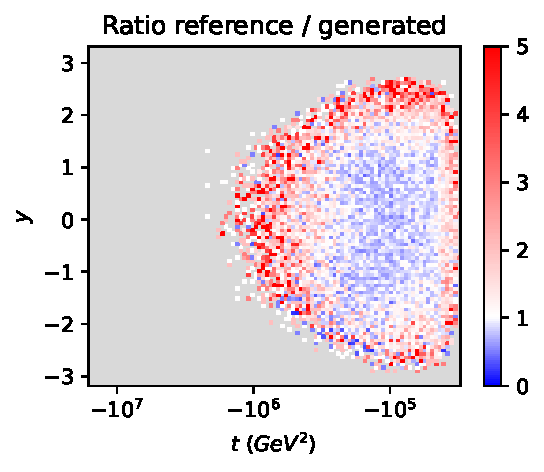
\includegraphics[width=0.33 \textwidth]{figures/plots/hardware/ibm_santiago/t-y_RATIO_IBM_100k.pdf}
        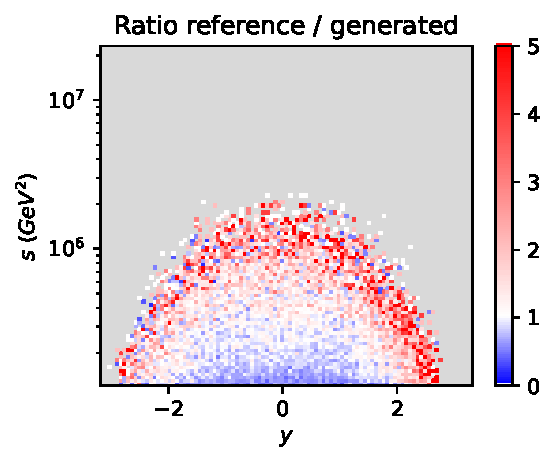
\includegraphics[width=0.33\textwidth]{figures/plots/hardware/ibm_santiago/y-s_RATIO_IBM_100k.pdf}
    \end{multicols*}
\end{frame}

\begin{frame}{Testing different architectures}
    \begin{multicols*}{2}
        Access constraints to ionQ: test limited to 1000 samples only
        \begin{tcolorbox}
           Hardware independent implementation!
        \end{tcolorbox}
    \end{multicols*}
    \begin{multicols*}{4}
        \textbf{IBM Q samples}
        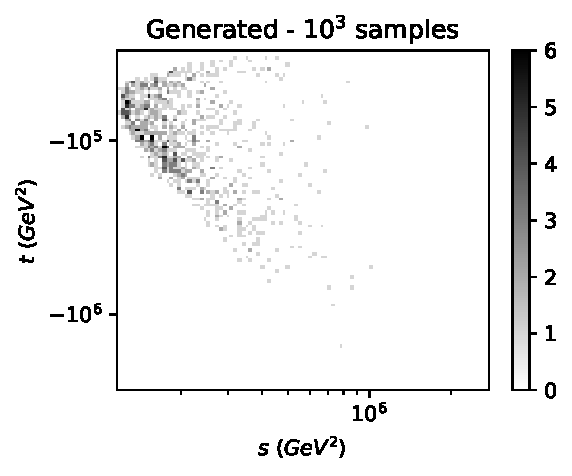
\includegraphics[width=0.25\textwidth]{figures/plots/hardware/ibm_santiago/s-t_FAKE_IBM_1k.pdf}
        \includegraphics[width=0.25 \textwidth]{figures/plots/hardware/ibm_santiago/t-y_FAKE_IBM_1k.pdf}
        \includegraphics[width=0.25\textwidth]{figures/plots/hardware/ibm_santiago/y-s_FAKE_IBM_1k.pdf}
    \end{multicols*}

    \begin{multicols*}{4}
        { \vfill 
        \textbf{ionQ samples}
        }
        \includegraphics[width=0.25\textwidth]{figures/plots/hardware/ionQ/s-t_FAKE_ionQ_1k.pdf}
        \includegraphics[width=0.25 \textwidth]{figures/plots/hardware/ionQ/t-y_FAKE_ionQ_1k.pdf}
        \includegraphics[width=0.25\textwidth]{figures/plots/hardware/ionQ/y-s_FAKE_ionQ_1k.pdf}
    \end{multicols*}
\end{frame}

\section{Outlook}
\begin{frame}{Outlook}
    \begin{itemize}
        \item A novel \textbf{quantum generator architecture} (style-based) has been presented.
        \item A test-case with real Monte Carlo event has demonstrated success: the generator has
        learned underlying $(s, t, y)$ distributions and correlations for production.
        \item Demonstrated \textbf{data augmentation} from $10^4$ training data to $10^5$ generated data.
        \item The quantum network is \textbf{shallow}: great advantage in the current NISQ era.
        \item Tested on two different quantum architectures: superconducting qubits (IBM) and
        trapped ions (ionQ) with similar performances. The quantum generator seems quite
        hardware-independent.
    \end{itemize}
\end{frame}

\end{document}